\documentclass[a4paper,utf8]{article}
\usepackage{default}
\usepackage{tipa}
\usepackage{lingsty}
\usepackage{graphicx}
\usepackage{ipashortcuts}
\usepackage{rotating}
\usepackage{subfigure}
\usepackage[authoryear]{natbib}
\setlength{\bibsep}{0.05cm}
%opening
\title{The Sri Lankan linguistic ecology}
\author{Sebastian Nordhoff}
 

\begin{document}

\maketitle

\section{Introduction}
\begin{itemize}
 \item The languages of Sri Lanka are of very similar typological markup
 \item Sinhala (14M), Tamil (2,9M), Malay (50k), Portuguese (very few, 2001 census)
 \item English, Vedda not treated here\
 \item These languages form the Sri Lankan sprachbund \citep{Bakker2006}
 \item idea: the languages converge
 \item question: what does it mean to converge?
\end{itemize}

\section{What does convergence mean?}
\begin{itemize}
 \item two possibilities
 \item a) all language become more like each other 
  \begin{itemize}
  \item Balkans
  \item multidirectional convergence
  \end{itemize}
 \item b) one language is the target towards which the other language(s) converge(s) 
  \begin{itemize}
  \item target variety is inert, e.g. Immigrant Englishes in the US
  \item  unidirectional convergence
  \end{itemize}
 \item Which kind of convergence are we dealing with in the Sri Lankan context? And are we dealing with convergence at all?
\end{itemize}
 
\begin{figure}
 \centering
 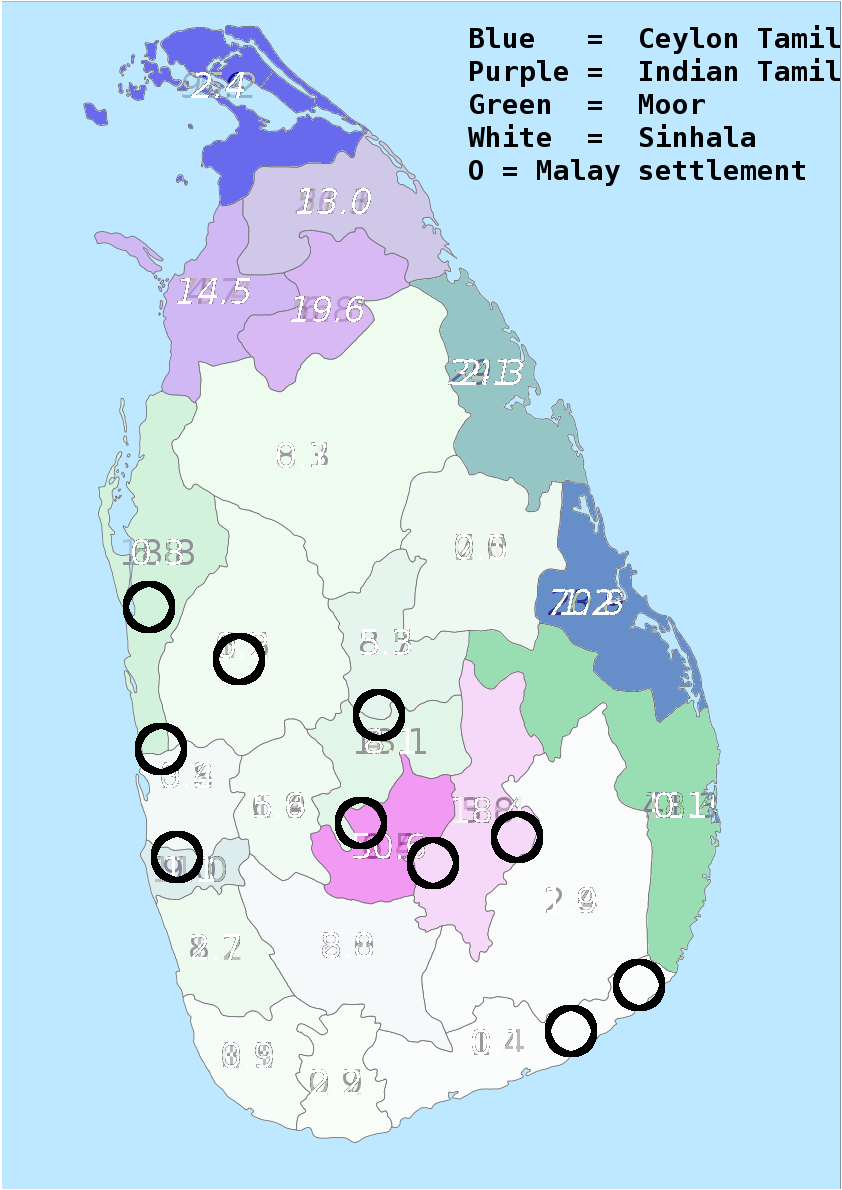
\includegraphics[height=.4\textheight]{./srilankacomposite.png}
 % srilankacomposite.png: 842x1190 pixel, 90dpi, 23.77x33.59 cm, bb=
 \caption{Geographical distribution of Sri Lankan populations}
\end{figure}

\newpage
\section{Sinhala: Should I stay or should I go}
 
\begin{itemize}
 \item  Sinhala is quite deviant from the Nothern Indian languages
\begin{itemize}
 \item long \=e, \=o
 \item no aspirated stops p$^h$ t$^h$ k$^h$ b$^h$ d$^h$ g$^h$  etc \citep{Elizarenkova1972}
 \item no postposed relative clauses \citep[507]{Geiger1973}\citep[204]{Gair1998someremarks}
 \item focus construction \citep{Gair1985calque}
 \item ``[S]ubordinate verbal structures as a whole are of a strikingly Tamil and Dravidian character ...  the cumulative effect is nothing short of overwhelming'' \citep{Gair1998someremarks}
\item quotative \citep{Gair1998someremarks}
%  \item no copula
\end{itemize}
 \item in fact, the membership of Sinhala in Indo-Aryan was contested in the 19th century \citep{Tennent1859,Prakasar1936,Prakasar1937,Geiger1938,Geiger1973}%g:495
\end{itemize}

\begin{itemize}
 \item SL Tamil is archaic \citep{Zvelebil1959II}
 \item SL Tamil has not changed a lot
 \item received opinion: Sinhala has converged towards Tamil
 \item uncontested for morphosyntax
 \item but the phonological picture is less clearcut \citep{Gair1985dravidianization}
\end{itemize}

\begin{table}[h]
\begin{tabular}{lll}
Pre-Old-Sinhala & Loss of aspiration & Tamil\\
 & Assimiliation in clusters & un-Tamil\\
Before 8$^{th}$ century & Simplification of geminates & un-Tamil\\
 & Metaphony/vowel fronting & un-Tamil\\
 & Word-final vowels merge as  /a/ & un-Tamil\\
 & s$>$h & un-Tamil(?)\\
 & c$>$s & Tamil(?)\\
About 8$^{th}$ century & Loss of vowel length & un-Tamil\\
 & Loss of final vowel with resultant final obstruents & un-Tamil\\
 & Loss of final v & Tamil\\
 & Loss of final y & un-Tamil\\
 & Reinstitution of vowel length & Tamil\\
After 8$^{th}$ century & Final nasals merge as [\ng] & un-Tamil\\
 & Reintroduction of geminates & Tamil\\
 & loss of \lz, \nz & un-Tamil
\end{tabular}
\caption{Phonological changes in Sinhala according to \citep{Gair1985dravidianization}}
\end{table}

\begin{itemize}
 \item It appears that Sinhala does not really know whether it wants to Tamilize or not. The case for convergence is not clearcut then, at least in the phonological domain
 \item And if Sinhala converged, what would it converge to?
\end{itemize}


\section{Tamil: Divergent structures in a linguistic area}

 
\begin{itemize}
 \item what Tamil are we talking about?
  \begin{itemize}
   \item ``Standard (Indian) Tamil''? \citep{Schiffman1999}
   \item ``In Sri Lanka, the notion of accepting or not accepting  the ``unifying'' ability of S[tandard] S[poken] T[amil] is another matter, since SST is understood but not accepted as an intercaste mode of communication among Sri Lankan Tamils. This matter will not be resolved until the civil war in that island has ended.'
   \item Sri Lanka Tamil
     \begin{itemize}
   \item ``Standard Sri Lanka Tamil''?
   \item \citet[170f]{Gairdonotuse}: ``There is, in fact, more dialect variation within  Tamil in Sri Lanka than there is within the majority (Indo-Aryan) language Sinhala.''
   \item ``It happens  quite frequently that, when speaking about  Ceylon(ese) Tamil, what authors have really in mind is (one dialect of ) \em Jaffna \em Tamil. This should of course be avoided''\citep[137]{Zvelebil1966} 
     \end{itemize}
  \end{itemize}
\item contrasts with Sinhala: ``We can hardly speak of any dialectal difference of the Sinhalese language in the Island itself''\citep[168]{Geiger1938}
\end{itemize}

\begin{figure}
\centering
 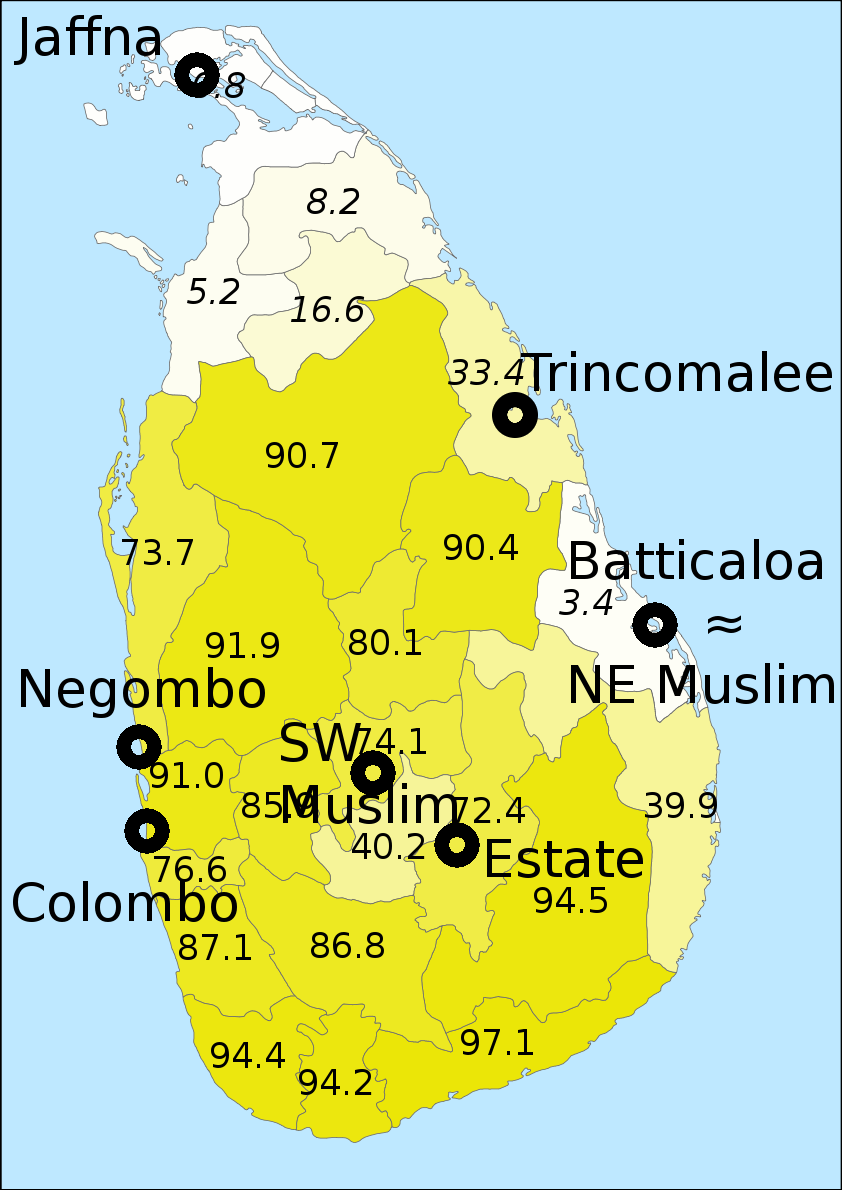
\includegraphics[height=.4\textheight]{describedtamildialects.png}
 \caption{Described dialects of Tamil. Shading and percentage indicate amount of Sinhala speakers in the area}
\end{figure}


\begin{itemize}
\item The ethnography of Tamil in Sri Lanka
  \begin{itemize}
  \item conservative
    \begin{itemize}
    \item Jaffna: prestigious, Christian/Hindu \citep{Zvelebil1959II,Kuiper1962,Pillai1962,Zvelebil1966,GairEtAl1979textbook,Gairdonotuse}
    \item Trincomalee: Hindu  \citep{Zvelebil1959I,Zvelebil1966}
    \item Batticaloa:  Hindu (literary-like)/Muslim \citep{Zvelebil1966,Batticaloa}
    \end{itemize}
  \item new
    \begin{itemize}
      \item mixed common Ceylonese \citep{Zvelebil1959II,Zvelebil1966}
    \end{itemize}
  \item deviant
      \begin{itemize}
      \item Negombo: no person inflection \citep{Bonta2004,Bonta2008}
      \end{itemize} 
 \item Muslim Tamil \citep{Nuhman2007}
\begin{itemize}
 \item North Eastern Muslim Tamil: conservative
 \item South Western Muslim Tamil: convergence towards Sinhala
 \begin{itemize}
  \item loss of inflection; loss of retroflex \nz{} and \lz{} \citep{Nuhman2007}
 \end{itemize}
 \item immigrant Tamil  
 \begin{itemize}
  \item Estate Tamil: Indian features (onglides, syncopation) \citep{Gairdonotuse,Wijeratne2005}
 \end{itemize}
\item What would be the `target variety', if any, for convergence?
\end{itemize}
\end{itemize}
\end{itemize}

% \begin{figure}
%  \centering
%  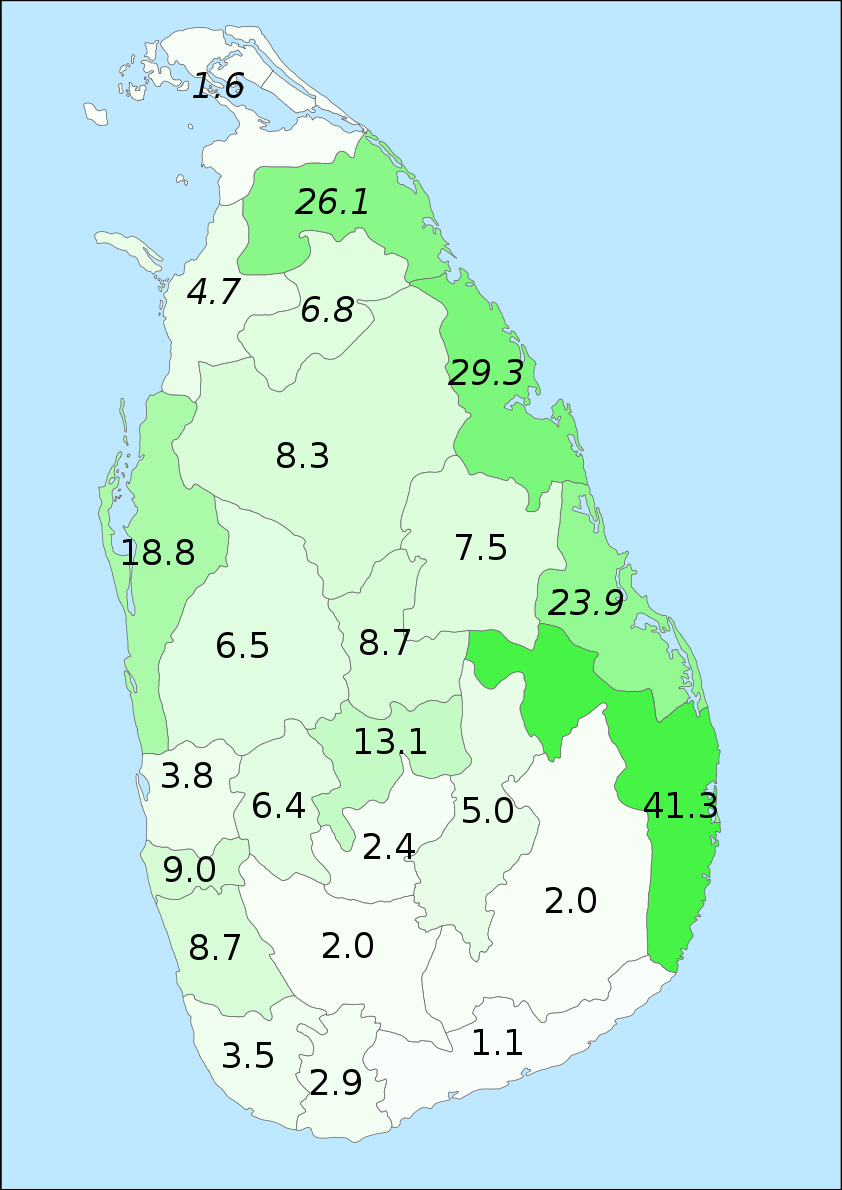
\includegraphics[width=.4\textwidth]{SriLankaMoor.png}
% \caption{Moor population in Sri Lanka}
% \end{figure}




\begin{figure}[h]
 \centering
 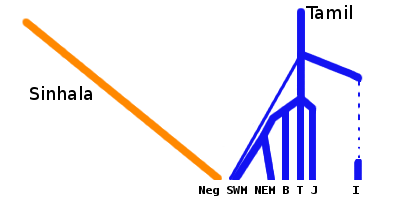
\includegraphics[width=\textwidth]{./Tamiltree.png}
 \caption{The convergence of certain varieties of Tamil towards Sinhala (Negombo, South Western Muslim Tamil, North Eastern Muslim Tamil, Batticaloa, Jaffna, Trincomalee,  Indian Estate Tamil).}
\end{figure}

\newpage
\section{Sri Lanka Malay: catch me if you can}

 
    \begin{itemize}
 \item SLM has become more South Asian
 \item Sinhala and Tamil share many structures \citep{Smith2003timing}
 \item What looks like Tamil influence could turn out to be Sinhala influence
 \item What looks like Sinhala influence could turn out to be Tamil influence
    \begin{itemize}
    \item If there is Sinhala influence on SLM, it could be called ``Dravidian through the back door'' because of earlier Tamilization of Sinhala
    \end{itemize}
\end{itemize} 
 
\begin{itemize}
 \item Which variety of Tamil is a contact language for SLM?
  \begin{itemize}
 \item The Malays had no contact to the more conservative varieties of Tamil because of geography
 \item Hindu or Christian prestige do not count for Malays (or Moors for that matter)
 \item contact varieties: generalized SL Tamil, Negombo Tamil, South West Muslim Tamil
 \item those are precisely the varieties that are Sinhalized
 \item the latter varieties' influence can be called ``Sinhala influence through the back door''
 \end{itemize}
\end{itemize} 

 
\begin{itemize}
 \item Cascading influences on Sri Lanka Malay: catch me if you can
    \begin{itemize}
    \item Malay converges towards SW Muslim Tamil\\
    .\hspace{1cm}$\rightharpoonup$ SW Muslim Tamil converges towards Sinhala\\
    .\hspace{2cm}$\rightharpoonup$ Sinhala converges towards general Dravidian structure
    \end{itemize}
\end{itemize}

\begin{itemize} 
 \item Traditional definition of convergence: the involved varieties become more like each other
 \item Sri Lanka
 \begin{itemize}
  \item  at bird's eye view
 \begin{itemize}
  \item Sinhala goes Tamil
  \item Tamil remains inert
 \end{itemize}
 \item at closer view
  \begin{itemize}
   \item  Sinhala goes Dravidian
   \item Tamil varieties diverge and become \em less \em like each other
  \end{itemize} 
 \item Malay is in the middle of the confusion
\end{itemize}
\end{itemize}

\begin{figure}
 \centering
 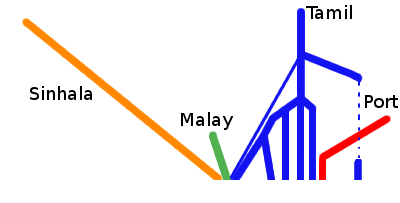
\includegraphics[width=\textwidth]{./lggraph.png}
\caption{Directions of language change in Sri Lanka}
\end{figure}



\begin{itemize}
 \item The moving target
  \begin{itemize}
  \item linear convergence is not an option for Malay because of the moving target
  \item Sri Lanka Malay targets Tamil varieties which are on their way towards Sinhala which is on its way to yet other Tamil varieties
  \item The simple solution ``Everybody goes Tamil, and so does Malay'' is conceptually simplistic and underestimates the internal complexity of Sri Lankan Tamil ethnography
  \item Tamil and Sinhala are already difficult to tell apart in their standard variety
  \item In this complex dialect situation, it is close to impossible to tease apart what is Sinhala and what is Tamil in the local languages, including Tamil and Sinhala
  \item For the time being, it seems advisable to take into account both Tamil and Sinhala features in analyzing SLM data, allowing for Tamil influence through Sinhala and Sinhala influence through Tamil
  \end{itemize}
\end{itemize}


\section{Conclusion}
\begin{center}
\begin{tabular}{lll}
conservative Tamil & = & conservative Tamil\\
Indian Tamil & $\to$ & Koineization\\
Sinhala & $\to$ & conservative Tamil\\
Muslim Tamil & $\to$ & Sinhala\\
Malay & $\to$ & Muslim Tamil, Sinhala
\end{tabular}
\end{center}



\begin{itemize}
 \item There is an `inert target', conservative Tamil: unidirectional convergence
 \item The `center of attraction'  or `typological mean'  seems to be somewhere between Sinhala and Muslim Tamil: multidirectional convergence
\end{itemize}

\nocite{Gair1998}
\bibliographystyle{natuva}
\bibliography{ansaldo,asw,creole,india,phon,malay,sinhala,tamil,nordhoff,lankahist}

\begin{figure} 
 \centering
\subfigure[Sinhala]{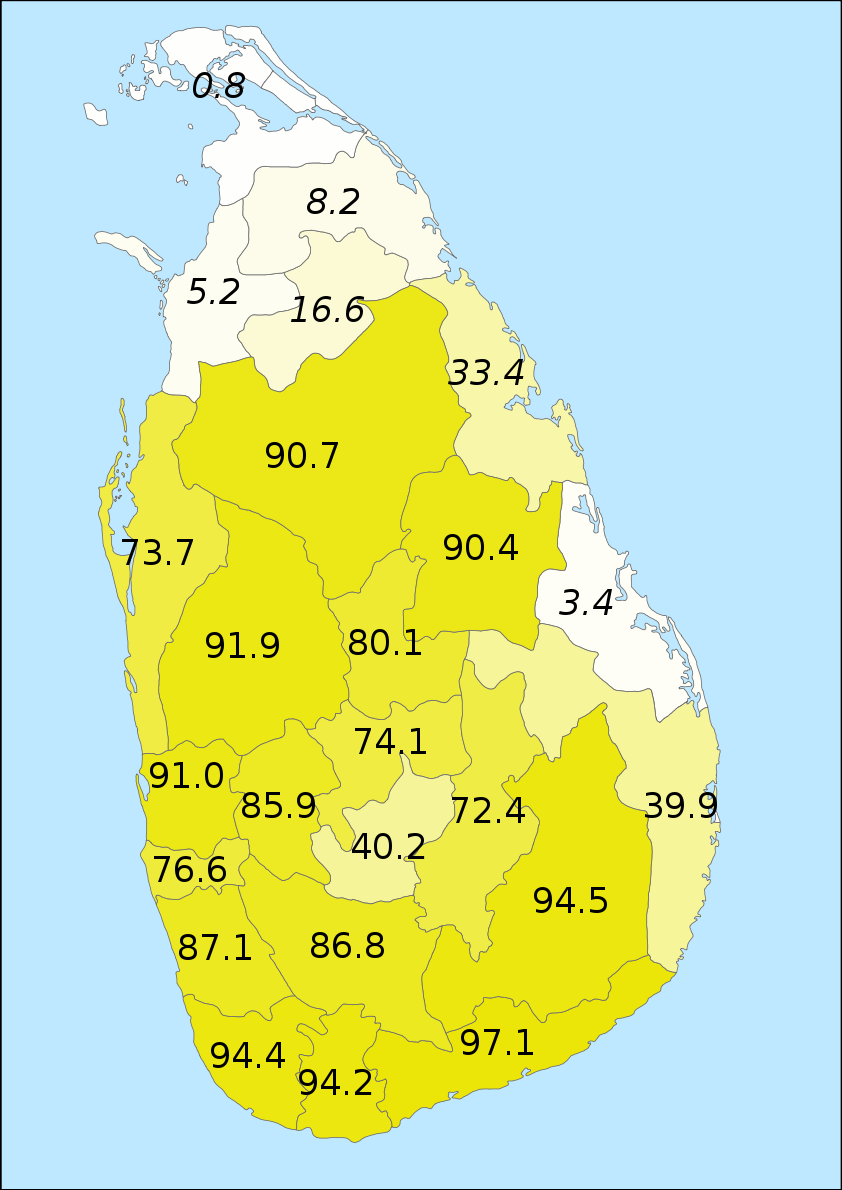
\includegraphics[width=.4\textwidth]{SriLankaSinhalese.png}}
\subfigure[Native Tamil]{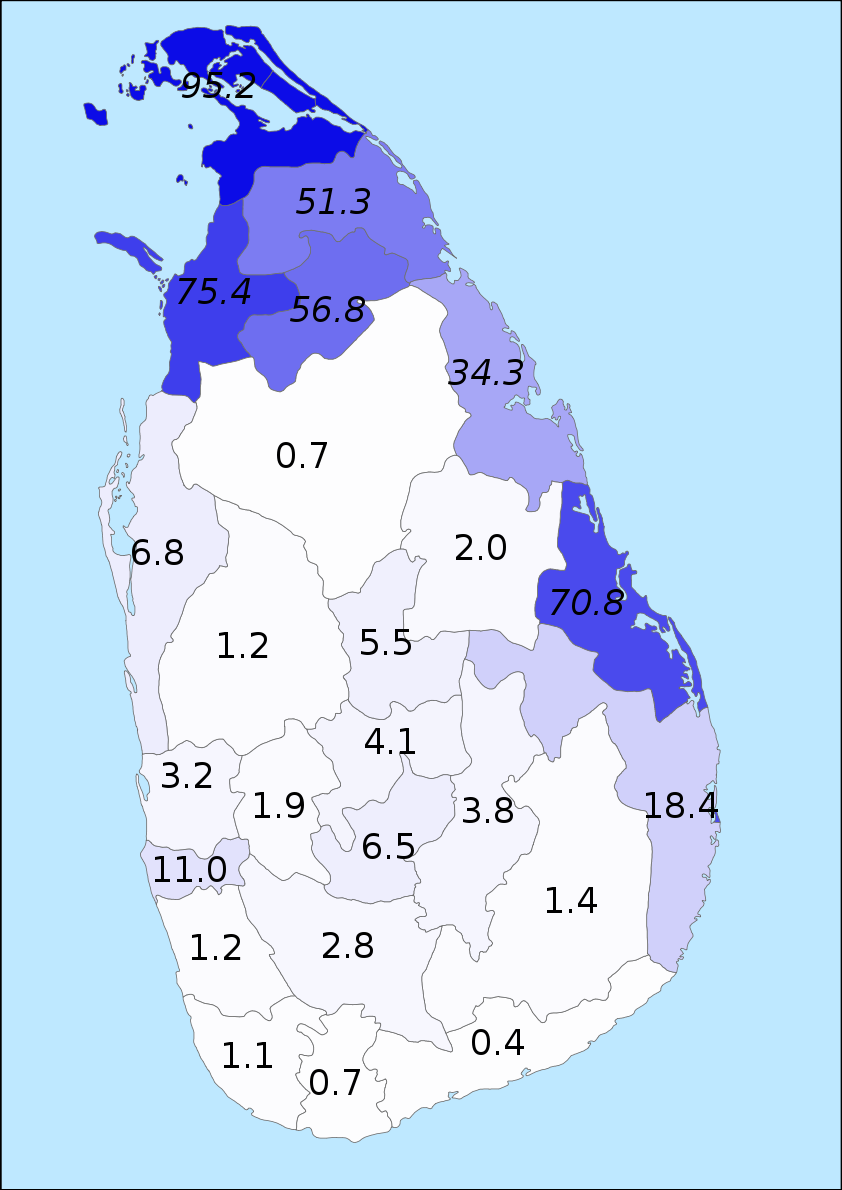
\includegraphics[width=.4\textwidth]{SriLankaNativeTamil.png}}

\subfigure[Indian Tamil]{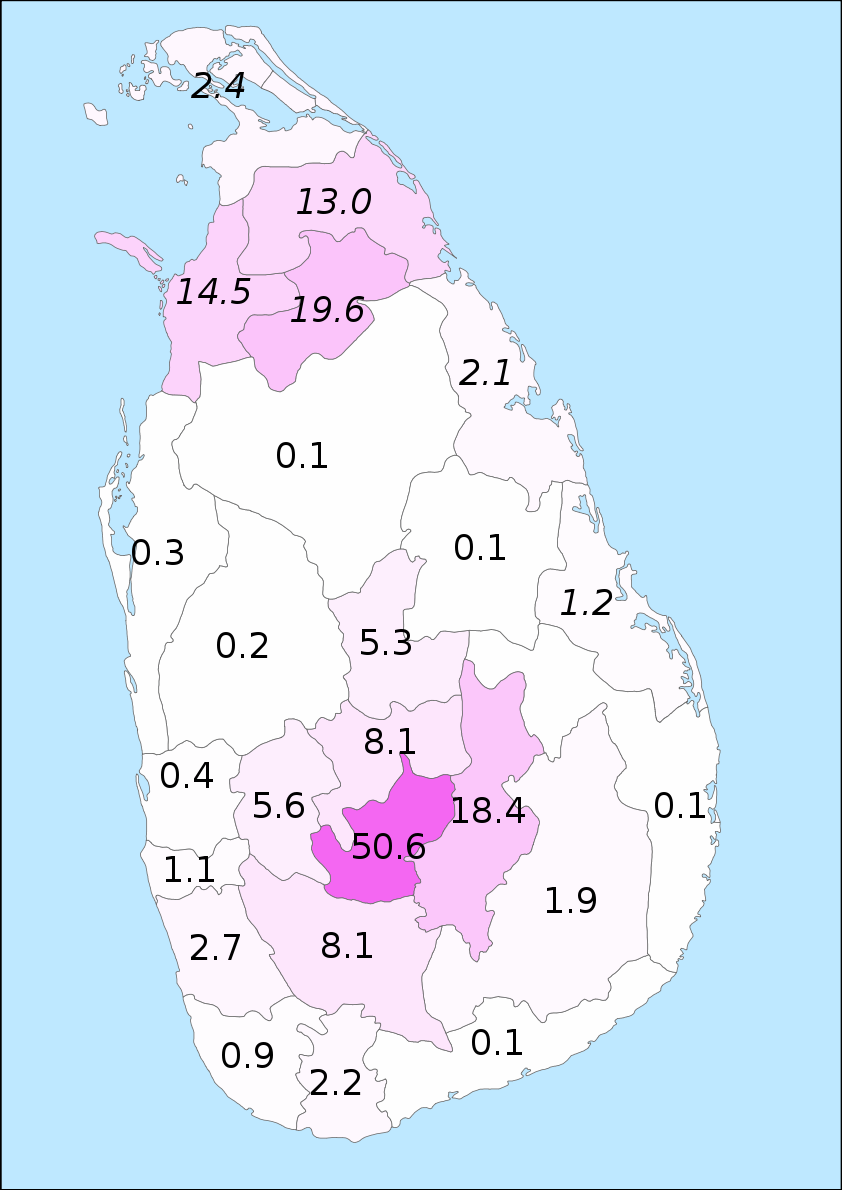
\includegraphics[width=.4\textwidth]{SriLankaIndianTamil.png}}
\subfigure[Moorsl]{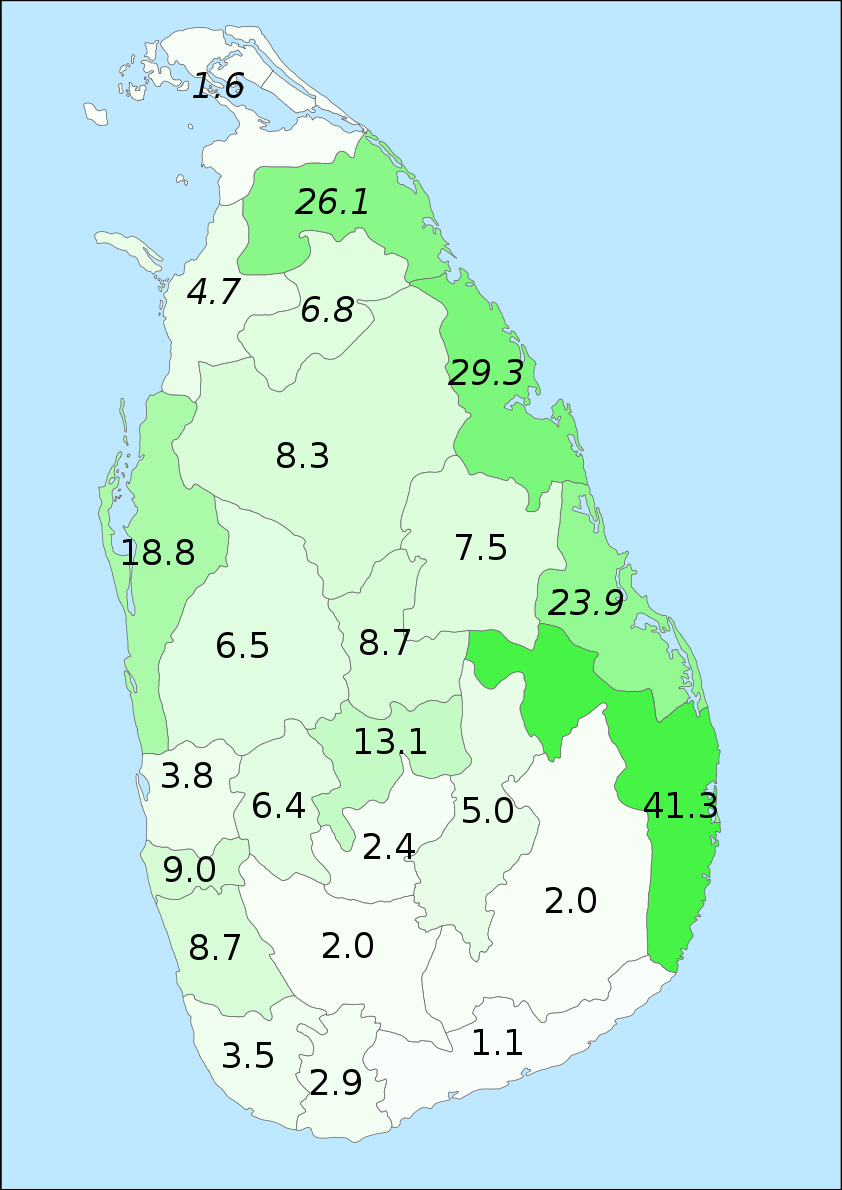
\includegraphics[width=.4\textwidth]{SriLankaMoor.png}}
\caption{Distribution of languages in Sri Lanka}
\end{figure}

  
\end{document}
